\pagestyle{fancy}
\headheight 20pt
\lhead{Ph.D. Thesis --- R. Woods}
\rhead{McMaster - Physics \& Astronomy}
\chead{}
\lfoot{}
\cfoot{\thepage}
\rfoot{}
\renewcommand{\headrulewidth}{0.1pt}
\renewcommand{\footrulewidth}{0.1pt}


\chapter{Code Tests}
\label{chap:codetests}
\thispagestyle{fancy}

In this chapter, I present a variety of tests to demonstrate the strengths and limitations of the above algorithm. Many test cases have been drawn from previous RT papers including \citet{ilievEt06,gendelevKrumholz12,skinnerOstriker13}. This chapter also include tests of accuracy and scaling of the algorithm.

\section{Glass}
\label{sec:glass}

A glass of particles is a simple way to demonstrate the most basic functionality of the algorithm. Each particle effectively acts to sample the radiation field at a particular point and has an easily calculated exact solution to compare to. A glass is also the relaxed state for an SPH simulation.

In the optically thin case, we simply want to ensure that we obtain a $1/r^2$ dropoff with flux. There should be no errors present in this test case because in the case of a single source, no averaging is needed and both exact luminosity and position of the source is used for every sink.

\begin{equation}
\label{eq:r2flux}
F = \frac{L}{4\pi r^2}
\end{equation}

In the case of absorption, the glass of particles has a roughly homogeneous density and thus the flux is still easily calculated for comparison.

\begin{itemize}
\item The equation for flux in this case is still fairly simple. If we refer to equation \ref{eq:radabsorption}, we can see the theoretical flux is simply equation \ref{eq:r2flux} multiplied by the exponential of optical depth. See equation \ref{eq:thickflux}.
\item This assumes a homogeneous density field. The glass does not have an exactly homogeneous field, but has little variance from the average.
\item Figure \ref{fig:thickglasserrors} shows the error distribution of the particles.
\item Note that in the case that the density field is exact, the errors reduce down to machine precision. This emphasizes the importance of accurately modeling the density distribution.
\end{itemize}

\begin{equation}
\label{eq:thickflux}
F = \frac{L}{4\pi r^2} \exp{-\tau}
\end{equation}

\begin{figure}
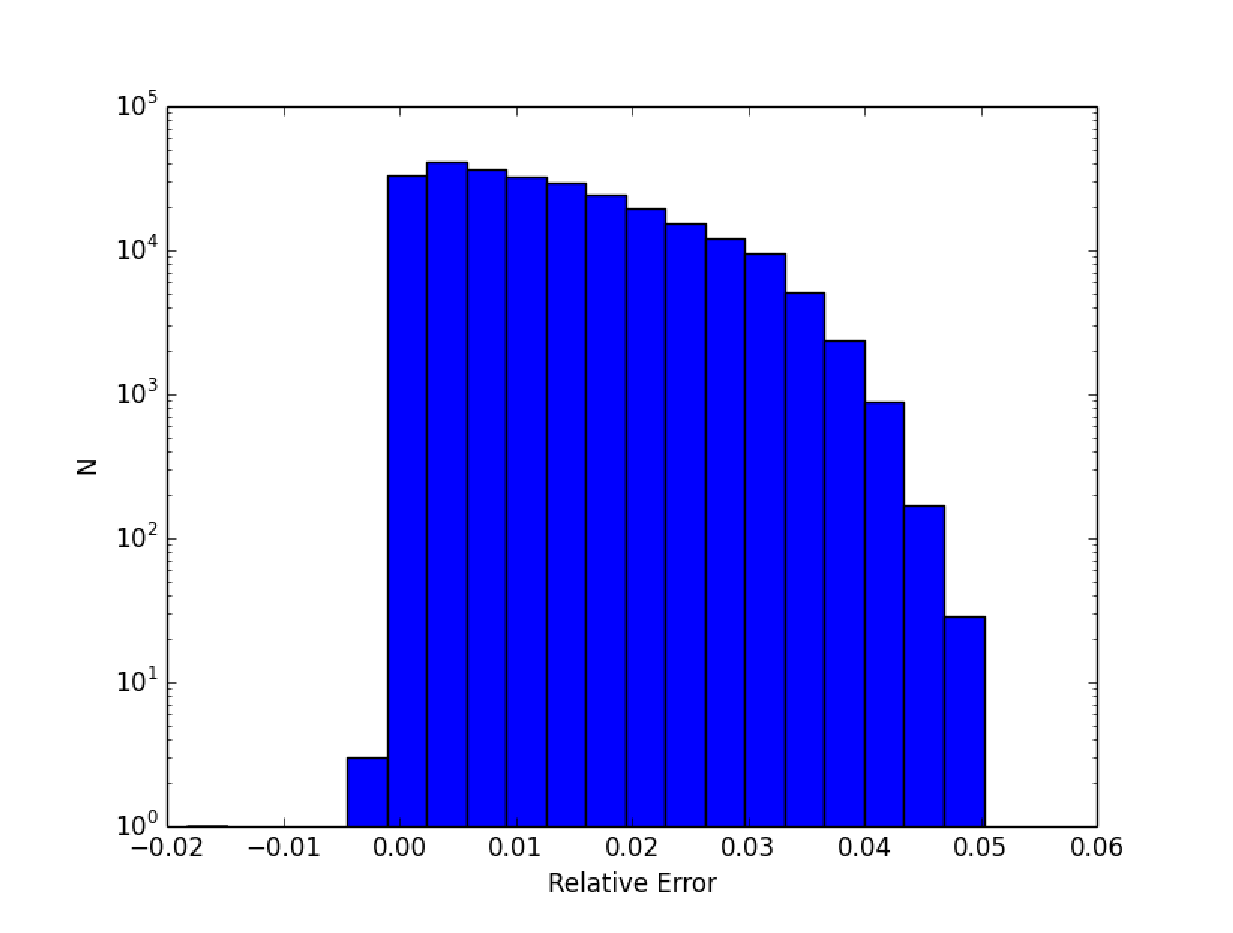
\includegraphics[width=\textwidth]{graphics/error.eps}
\caption[Error distribution for a single source in a uniform field.]{The distribution of flux errors among particles.}
\label{fig:thickglasserrors}
\end{figure}

\section{Multi-Source Glass}
\label{sec:multiglass}

We now show the effect of including many sources. The code is now performing at its most ``stressed;'' having a large number of randomly distributed sources means the code will run at its slowest and will include a large amount of averaging (not quite right).

\begin{itemize}
\item We first present the optically thin case. In this case, the glass has had half of its gas particles replaced with sources so that there are an equal number of each.
\item The error distribution present in this case demonstrates the errors associated with the tree method. [make mean error vs theta plot?]
\item 
\end{itemize}

\section{Effects of Averaging the Source}
\label{sec:averagingsource}

We now look closely at what effects averaging sources can have on results. To demonstrate this, we have created a box of gas with two stars placed offset from each other.

%\subsection{Two star}
%\label{sec:twostar}

\begin{figure}
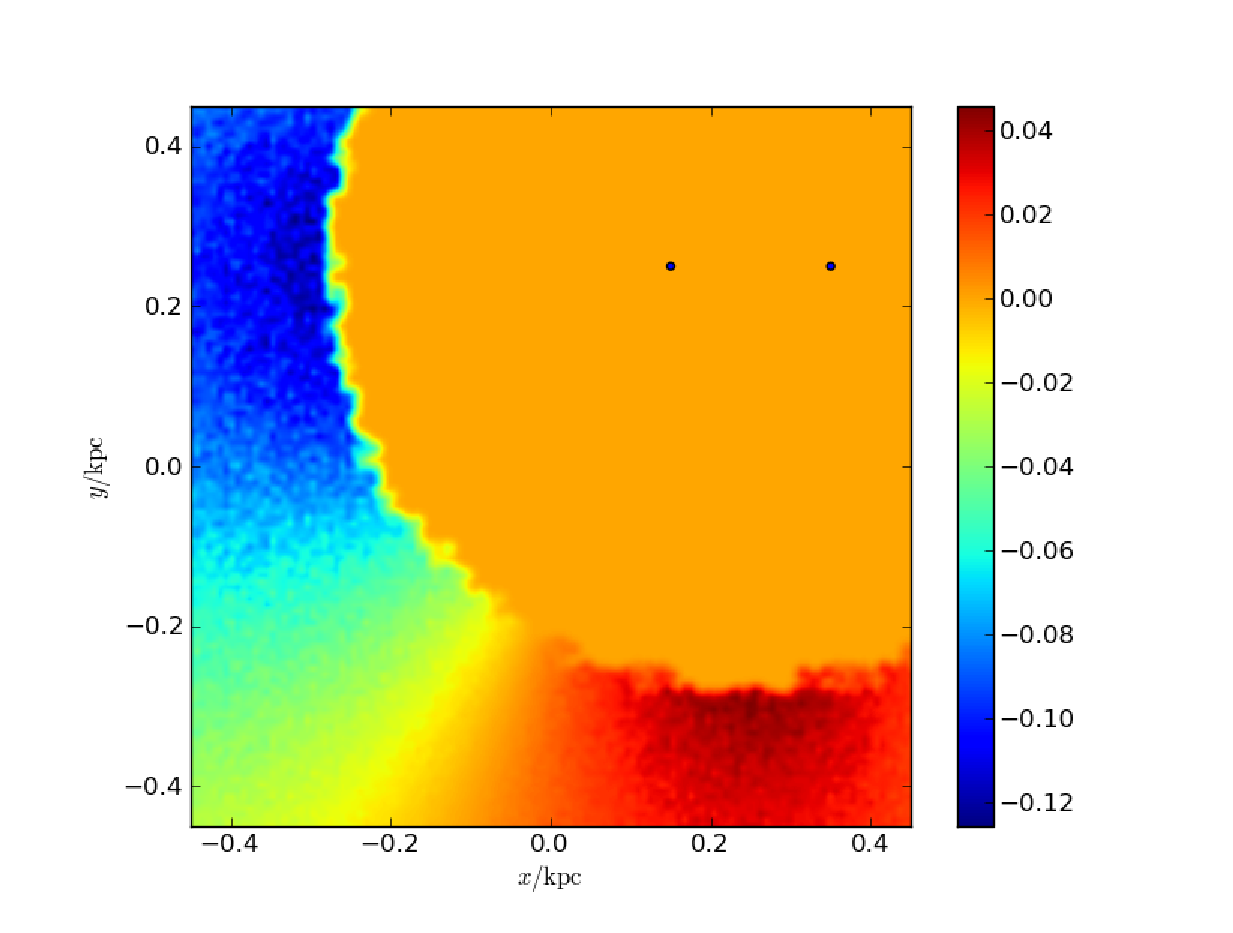
\includegraphics[width=\textwidth]{graphics/errorMap2starthick.eps}
\caption[The error associated with averaging star positions.]{The error associated with averaging star positions.}
\label{fig:twostar}
\end{figure}


%\subsection{Isothermal Sphere with a Cluster(?)}
%\label{sec:cluster}
%
%Words

\section{The Str\"omgren Sphere}
\label{sec:stromgren}

The str\"omgren sphere is a theoretical ionized sphere of gas. It was first discussed by Bengt Str\"omgren in 1938 \citep{stromgren39}. We start with a cloud of homogeneous neutral Hydrogen gas and an ionizing source, commonly representing an O or B-type star, at the center. As the photons from the source ionize the hydrogen, the optical depth of the gas decreases, and so the ionizing photons move further out creating an ionization front. As the front moves out, the photon density as a function of radius falls off simply due to $1/r^2$ geometry and eventually a point is reached where the ionization rate falls to the recombination rate. At this point, the front stops in equilibrium.

%One can solve for this radius by setting the photon density as a function of radius to the recombination rate and solving for radius \citep{stromgren39,spitzer78},
%
%\begin{equation}
%\label{eq:stromgrenradius}
%R_S = \left( \frac{3}{4\pi} \frac{\dot{N_{\gamma}}}{\alpha n_H^2}\right).
%\end{equation}
%
%One can also find the growth rate of the front,
%
%\begin{equation}
%\label{eq:stromgrentime}
%R(t) = R_S[1-\exp{(t/t_{\mbox{recomb}})}]^{1/3}.
%\end{equation}
%
%The above equations are the solutions for the evolution of a sharp ionization front, meaning that we have assumed the transition from ionized to neutral is infinitesimal in size. In order to solve for a non-sharp front, we must solve some equations numerically. FILL IN METHOD HERE.

\subsection{The Isothermal Case}
\label{sec:isostromgren}

In the simplest case, the ionizing source is assumed to emit photons at exactly 13.7 ev, meaning that the hydrogen gas is ionized but not heated. Cooling is also disabled, meaning that the gas is isothermal. If we assume that the ionization front propagates until the ionization rate drops low enough (due to geometric diminishment) to equal the recombination rate of the ambient medium, then we can solve for the equilibrium ionization radius by setting the two rates equal.

The ionization rate per unit volume can be written as the (fill in here)

%\begin{equation}
%\label{eq:fluxrecomb}
%F = \int_0^{r_s} n_e n_H \alpha_B(T) dl,
%\end{equation}
%
%where $n_e$ is the number density of electrons, $n_H$ is the number density of neutral Hydrogen, $\alpha_B$ is the case B recombination coefficient for Hydrogen for a given temperature, and $r_s$ is the equilibrium radius or ``Str\"omgren radius.'' 

\begin{equation}
\label{eq:strmogrenradius}
R_S = \left( \frac{3}{4\pi} \frac{\dot{N_{\gamma}}}{\alpha n_H^2}\right)
\end{equation}

\begin{equation}
\label{eq:stromgrentime}
R(t) = R_S[1-\exp{(t/t_{\mbox{recomb}})}]^{1/3}
\end{equation}

The above derivation assumes a ``sharp'' ionization front, meaning the transition from ionized to neutral is across an infinitesimal region. In practice, the transition region is small compared to the size of the ionized region, but there is structure interior to the Str\"omgren radius that is not accounted for by simply solving for the equilibrium radius. In order to solve for a non-sharp ionization front, we must integrate the above ionization equations \citep{osterbrockFerland2006}. (ADD HERE). In the following tests, we include both the sharp and non-sharp ionization front solutions for comparison to our results.

We follow the initial conditions of \citet{ilievEt06}; the medium is initially neutral with a temperature 1e5 K and a density of 1e-3 cm$^{-3}$. An ionizing source is turned on at t = 0 that emits $\dot{N} = 5e48$ photons s$^{-1}$ at 13.6 ev. We use a cross section $\sigma = 6.3e-18 cm^2$ and a recombination rate of $\alpha = 2.59e-13 cm^{-3} s^{-1}$, typical of 1e5 K gas. These values give a Str\"omgren radius of 5.38 kpc and a recombination time of 125 Myr.

\begin{figure}
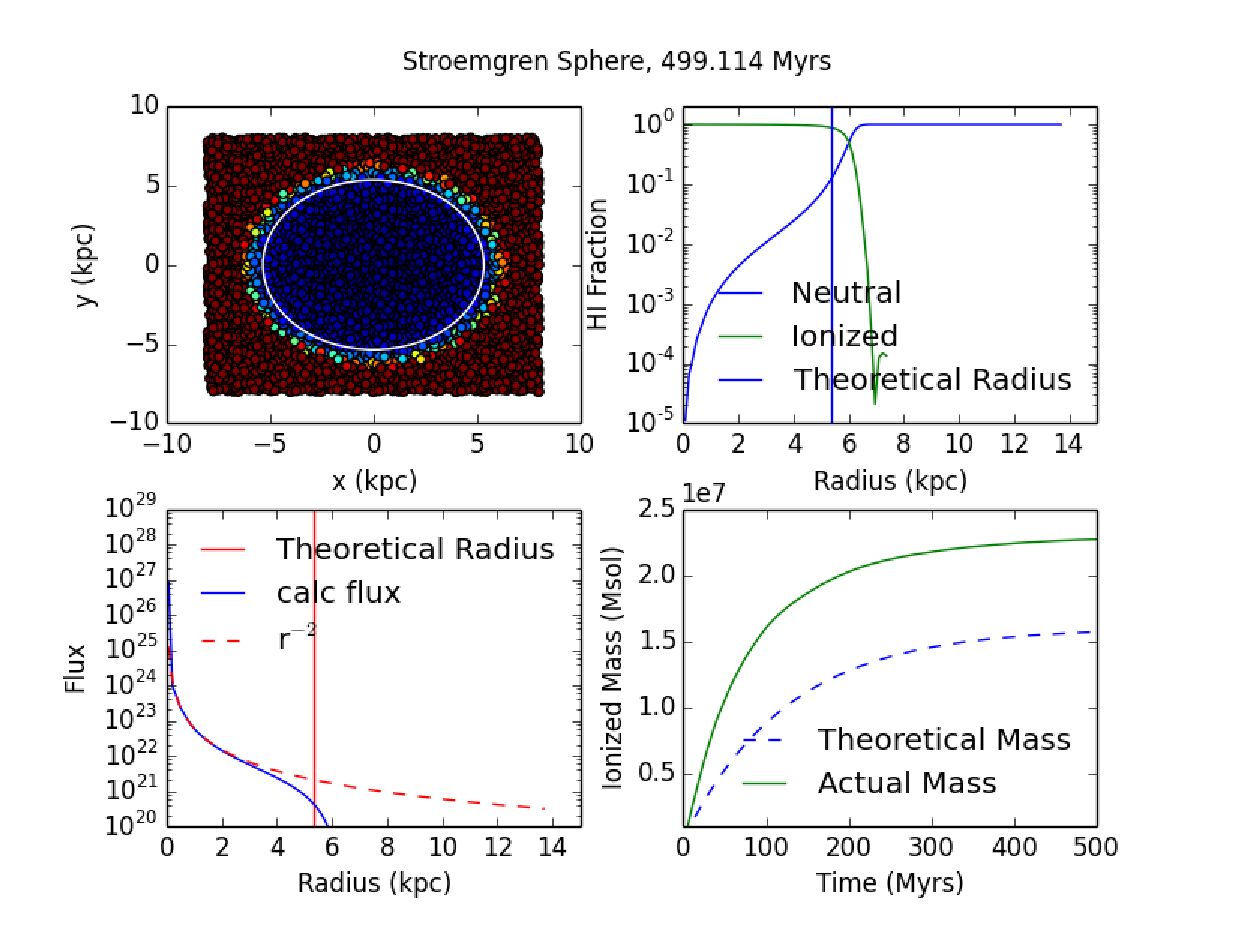
\includegraphics[width=\textwidth]{graphics/ifront6401000.eps}
\caption[The isothermal Str\"omgren Sphere.]{A slice of particles showing the ionization state.}
\label{fig:stromgreniso}
\end{figure}

\subsection{The Thermal Case}
\label{sec:thermalstromgren}

The above formulation assumed the gas was isothermal and that all incident photons had the same energy. In reality, photons range across many wavelengths (commonly in a Planck spectrum) with differing cross sections for each wavelength. As well, absorption typically causes heating, which effects, among many properties, recombination rate.

In order to do a more realistic test,the incident photons are assumed to be from a black body with temperature 1e5 K. The cross section is changed to an integrated cross section, obtained by integrating the cross section as a function of wavelength over all wavelengths having energies between 13.6 ev and 29.65 ev. The gas has an initial temperature, This scenario does not have an analytic solution to compare to, and so we instead compare to the results of \citet{ilievEt06} and \citet{petkovaSpringel09}. (NOTE - seems to be inconsistency. 10$^5$ K source corresponds to ~43 ev = 29.65 + 13.6, but other areas seem to indicate total energy of 29.65, not heating energy = 29.65. Figure this out).

This test includes heating due to absorption and cooling due to recombination $\Lambda_r$, collisional ionization $\Lambda_{ci}$, line cooling $\Lambda_l$, and Bremsstrahlung radiation $\Lambda_B$. The rate are taken from \citet{cen92} in order to match \citet{petkovaSpringel09}. The following are those rates in ergs cm$^{-3}$ s$^{-1}$:

\begin{align}
\label{eq:cencooling}
\Lambda_r & = {8.7\e{-27} \sqrt{T}\left(\frac{T}{10^3 K}\right)^{-0.2}} \Biggm/{\left[1+\left(\frac{T}{10^6 K}\right)^{0.7}\right]}, \\
\Lambda_{ci} & = 1.27\e{21} \sqrt{T}\left(1 + \sqrt{\frac{T}{10^5 K}}\right)e^{157809.1/T} n_e n_{HII},\\
\Lambda_l & = 7.5\e{-19}\left(1+\sqrt{\frac{T}{10^5 K}}\right)^{-1}e^{-118348/T}n_e n_{HI},\\
\Lambda_B & = 1.42\e{-27}g_{ff}\sqrt{T}n_e,
\end{align}

where $g_{ff} = 1.3$ is the gaunt factor.

\begin{figure}
        \centering
        \begin{subfigure}[b]{0.3\textwidth}
                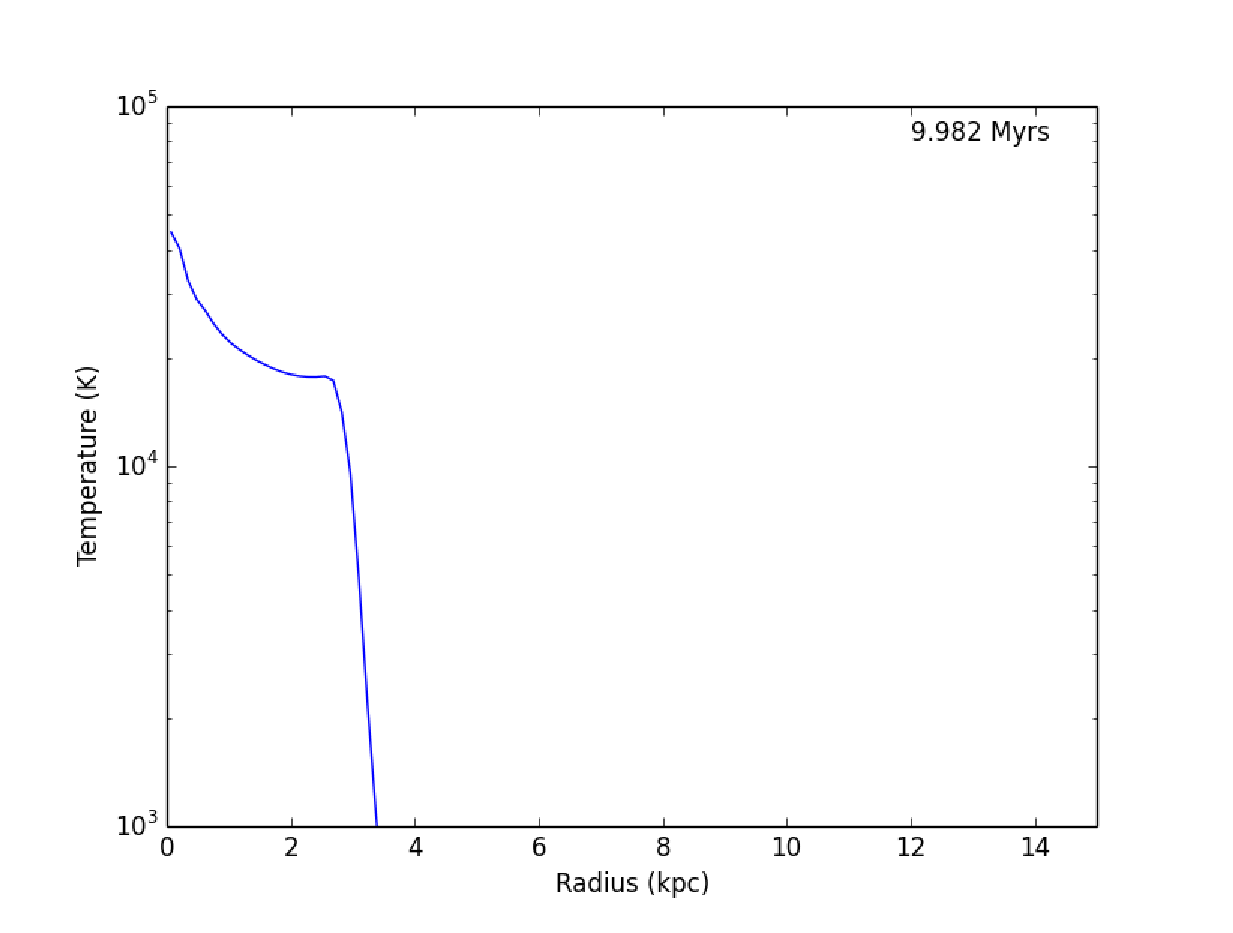
\includegraphics[width=\textwidth]{graphics/ifrontThermal6400020Tempprofile.eps}
                \label{fig:stromgrenthermal10}
        \end{subfigure}
        ~ 
        \begin{subfigure}[b]{0.3\textwidth}
                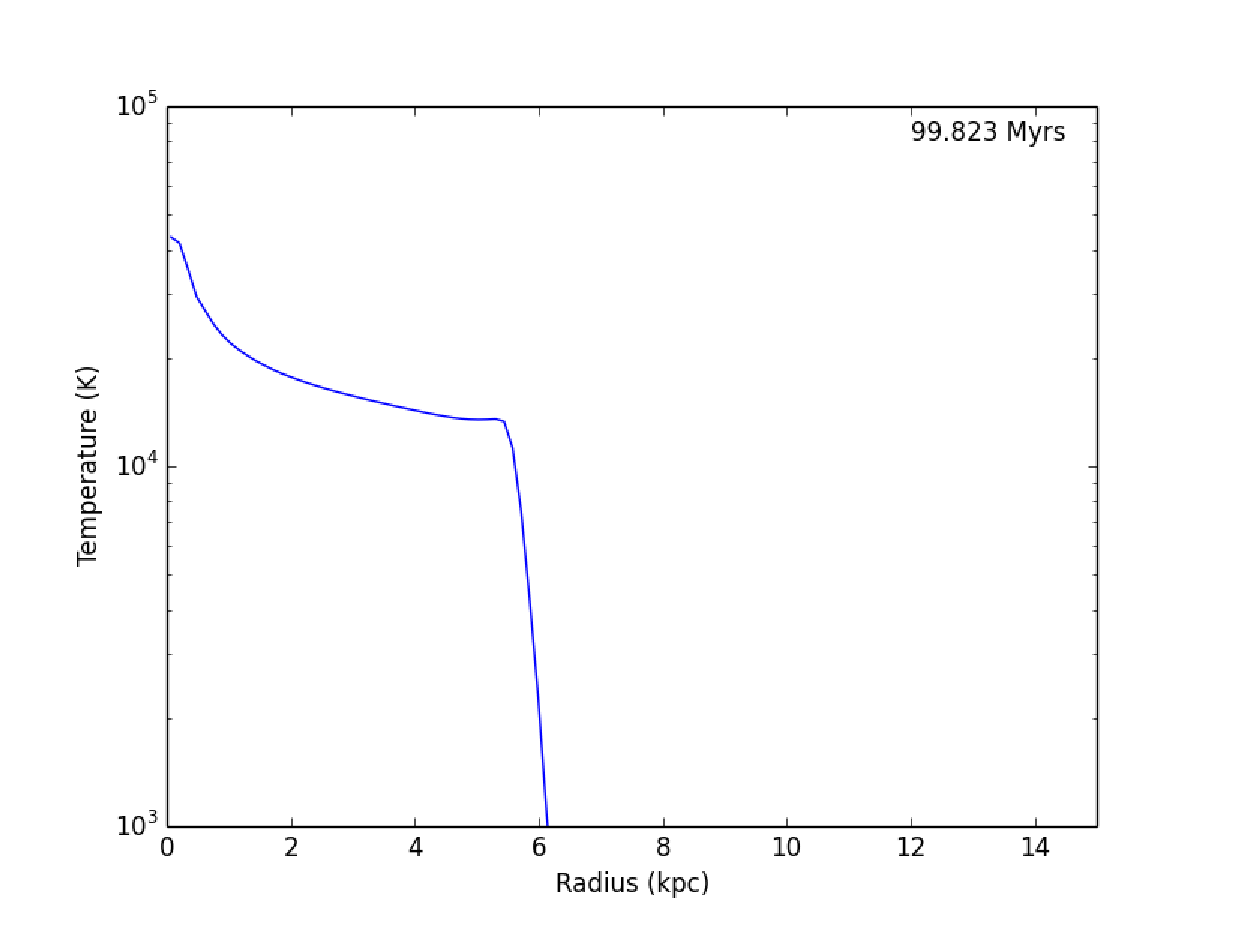
\includegraphics[width=\textwidth]{graphics/ifrontThermal6400200Tempprofile.eps}
                \label{fig:stromgrenthermal100}
        \end{subfigure}
        ~
        \begin{subfigure}[b]{0.3\textwidth}
                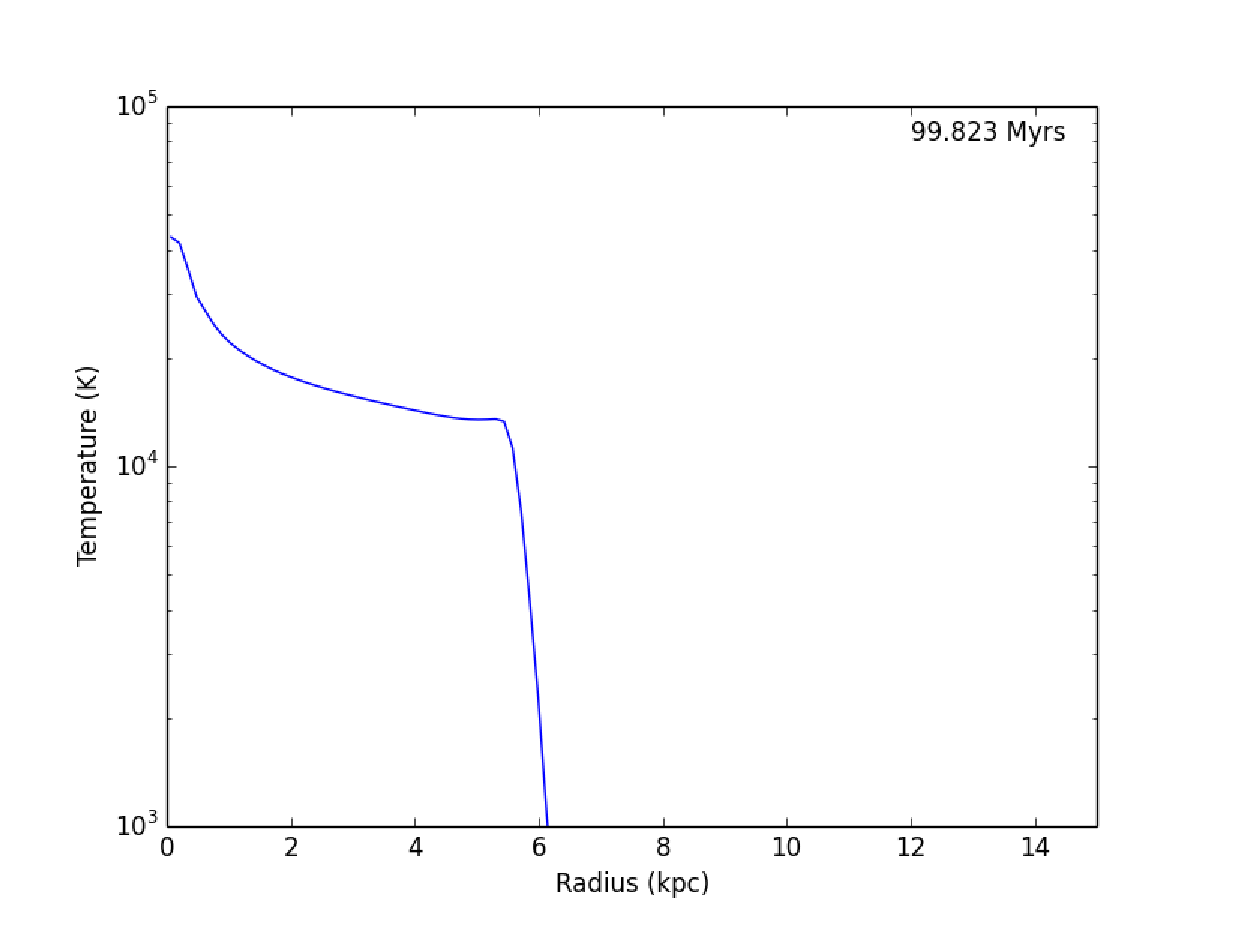
\includegraphics[width=\textwidth]{graphics/ifrontThermal6400200Tempprofile.eps}
                \label{fig:stromgrenthermal500}
        \end{subfigure}
        \caption[Temperature vs radius for the thermal Str\"omgren sphere.]{Temperature vs radius for the thermal Str\"omgren sphere.}
        \label{fig:stromgrenthermal}
\end{figure}

Figure \ref{fig:stromgrenthermal} shows a radially averaged profile of temperature. We see a peak temperature of roughly $3\e{4} K$ with a radial dropoff stimilar to results from \citet{ilievEt06}. This demonstrates the code's ability to couple radiation to the thermodynamics of the gas (ADD MORE).

\section{The Gas Wall}
\label{sec:gaswall}

In order to test the algorithm's ability to handle a sharp density jump, we again perform the isothermal stromgren front (section \ref{sec:isostromgren}), but with a large density jump. We keep all of the same initial parameters, but change the density to the left of x = 0 to $\rho/2$ and the density to the right of x = 0 to $3/2 \rho$.

\subsection{Only Radiation}
\label{sec:gaswallradonly}

In the case that hydrodynamics is off, the solution is two str\"omgren hemispheres centered at x = 0.

\begin{figure}
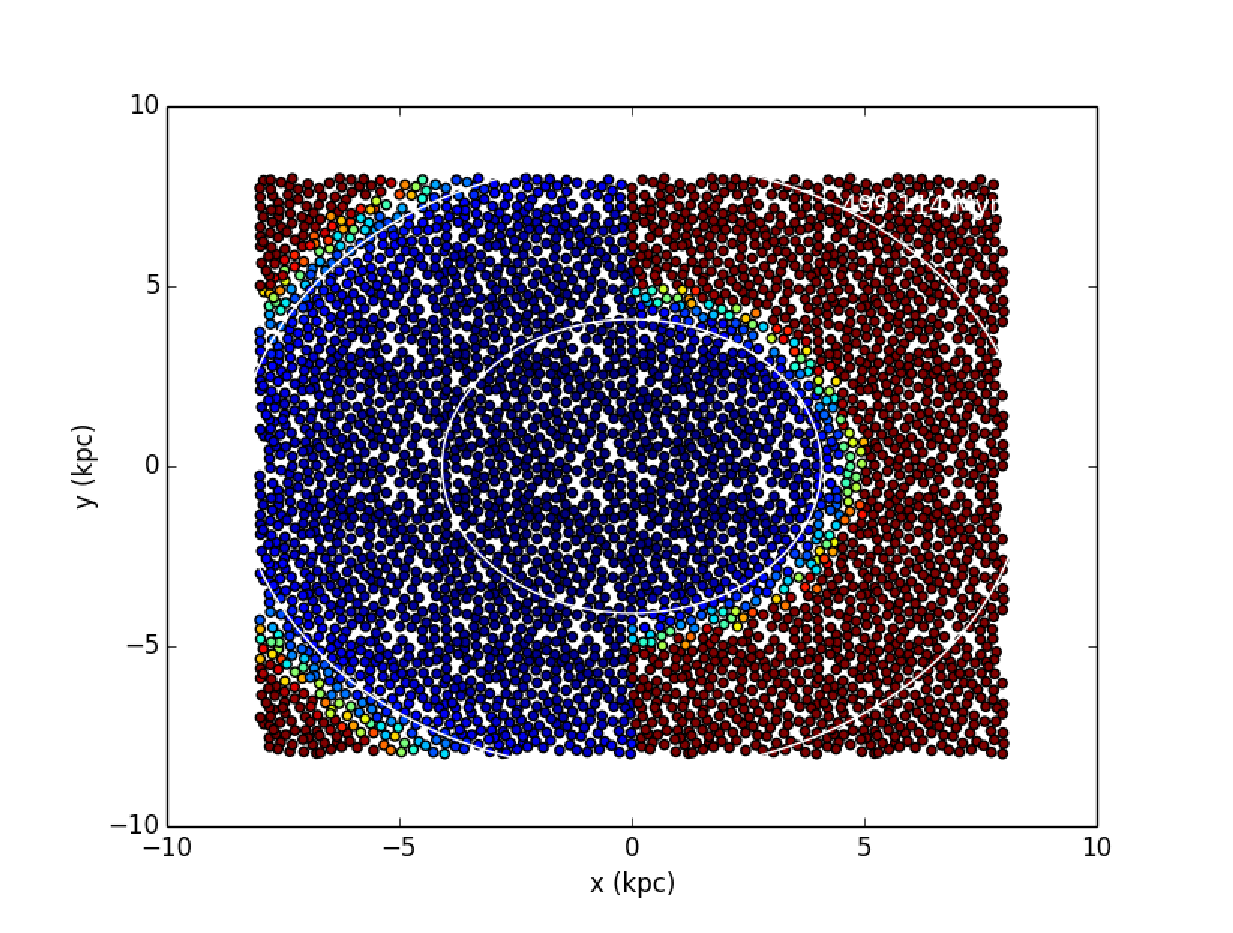
\includegraphics[width=\textwidth]{graphics/gasWall01000HIslice.eps}
\caption[Two slabs of gas at different densities.]{Two slabs of gas at different densities.}
\label{fig:gaswall}
\end{figure}


\subsection{With Hydrodynamics - the Champagne Flow}
\label{sec:champagne}

In order to test the coupling of radiation to the hydrodynamics, we perform a similar test in which the code now uses its hydrodynamics solvers. We follow the setup of \citet{gendelevKrumholz12}; A 50 pc cube is initialized with a density of 0.055 atoms cm$^{-3}$ to the right of x = 0, and 63 atoms cm$^{3}$ to the left. The temperatures of the left and right halves are 55 K and 6.3e3 K, respectively. This density/temperature combination gives pressure equilibrium at the boundary. An ionizing source is turned on at the origin that emits 5.3e47 photons/s, similar to a type BO.5 star. The combination of density and luminosity gives a stromgren sphere radius of 1.5 pc in the dense regio
ns and a recombination time of 2.48e4 Years. The simulation is run for more than 4e6 years, meaning that the gas has time to heat and expand.

\begin{figure}
        \centering
        \begin{subfigure}[b]{0.3\textwidth}
                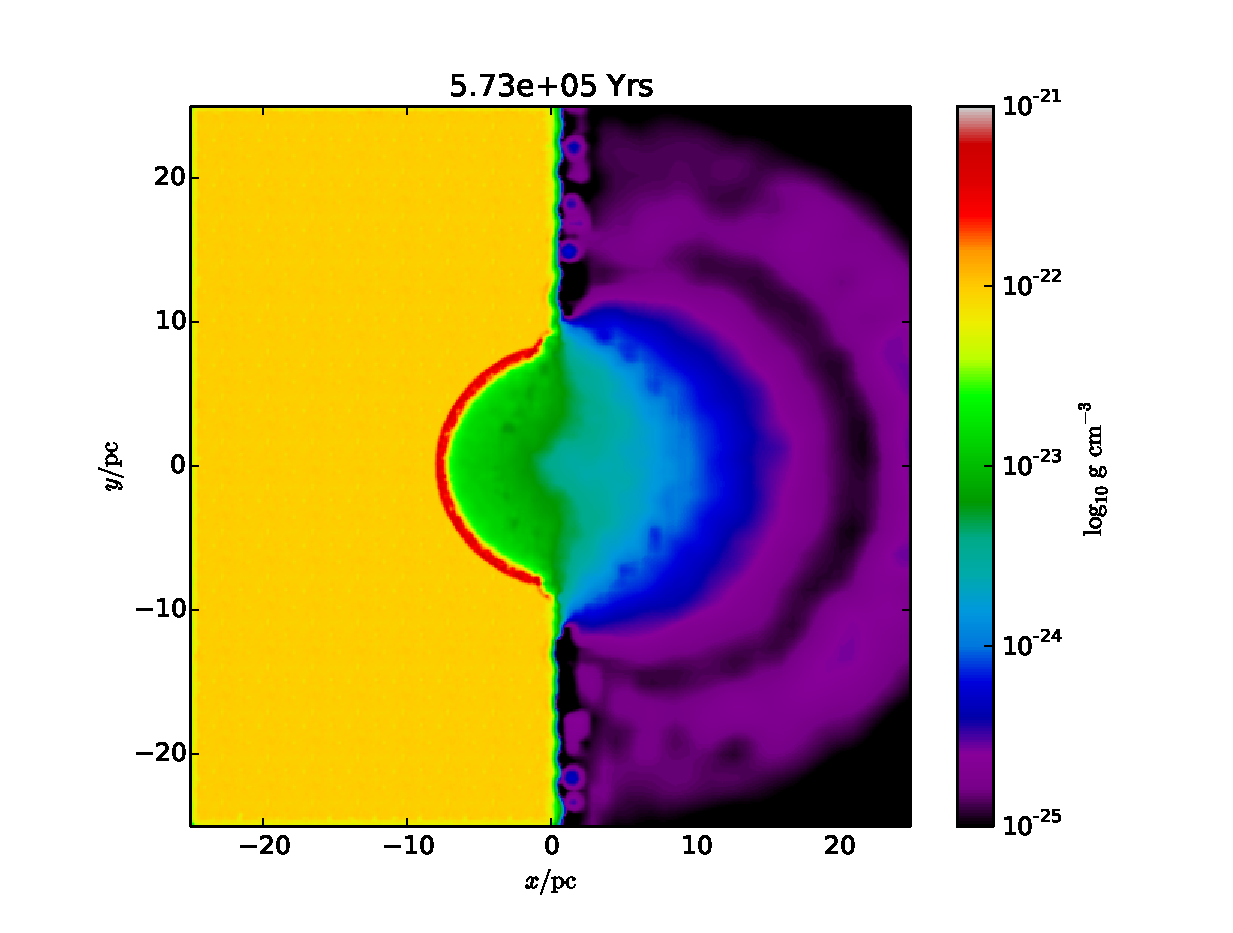
\includegraphics[width=\textwidth]{graphics/blister25600040rhoslice.eps}
                \caption{0.5 Myr}
                \label{fig:champagne1}
        \end{subfigure}
        ~ 
        \begin{subfigure}[b]{0.3\textwidth}
                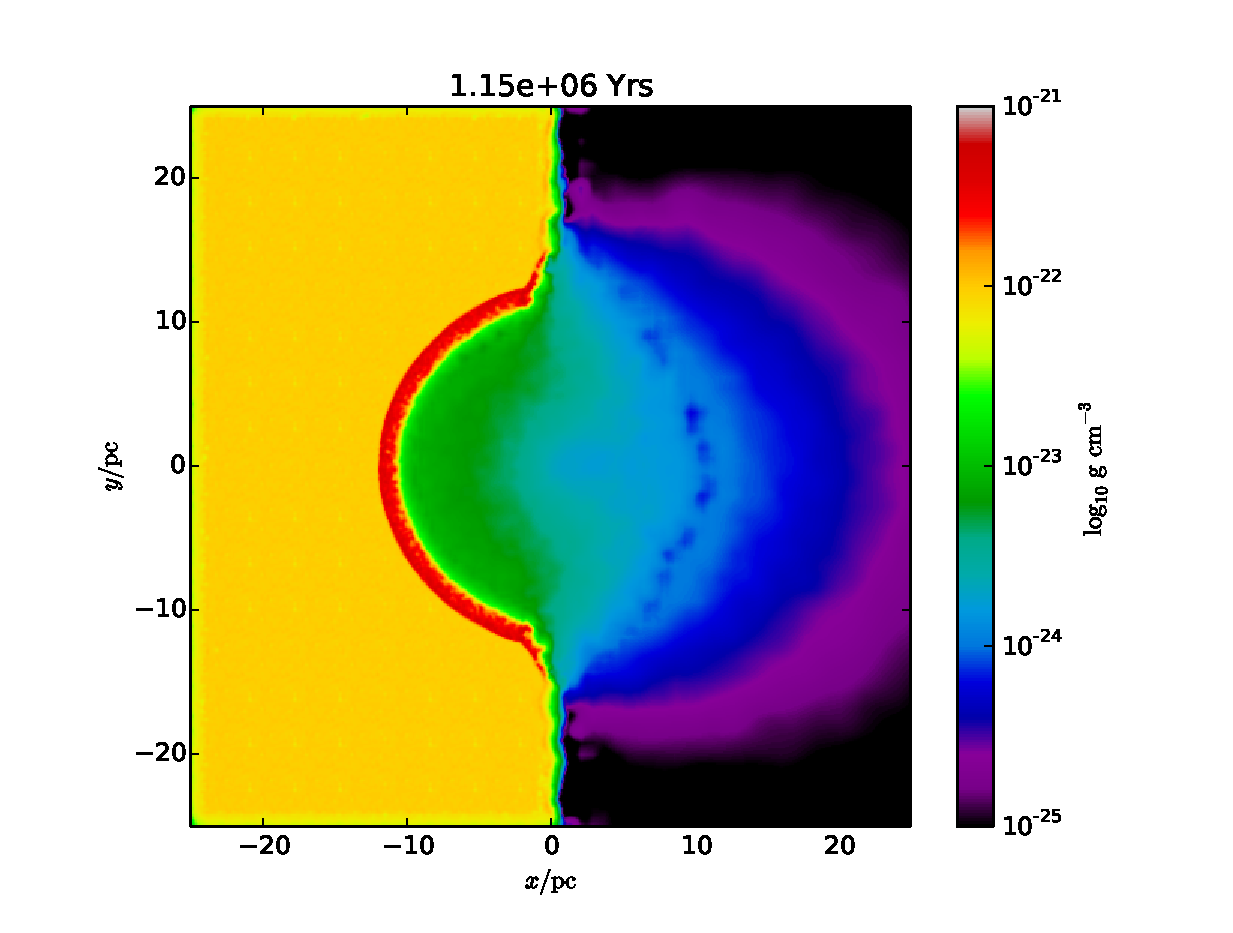
\includegraphics[width=\textwidth]{graphics/blister25600080rhoslice.eps}
                \caption{1 Myr}
                \label{fig:champagne2}
        \end{subfigure}
         ~ 
        \begin{subfigure}[b]{0.3\textwidth}
                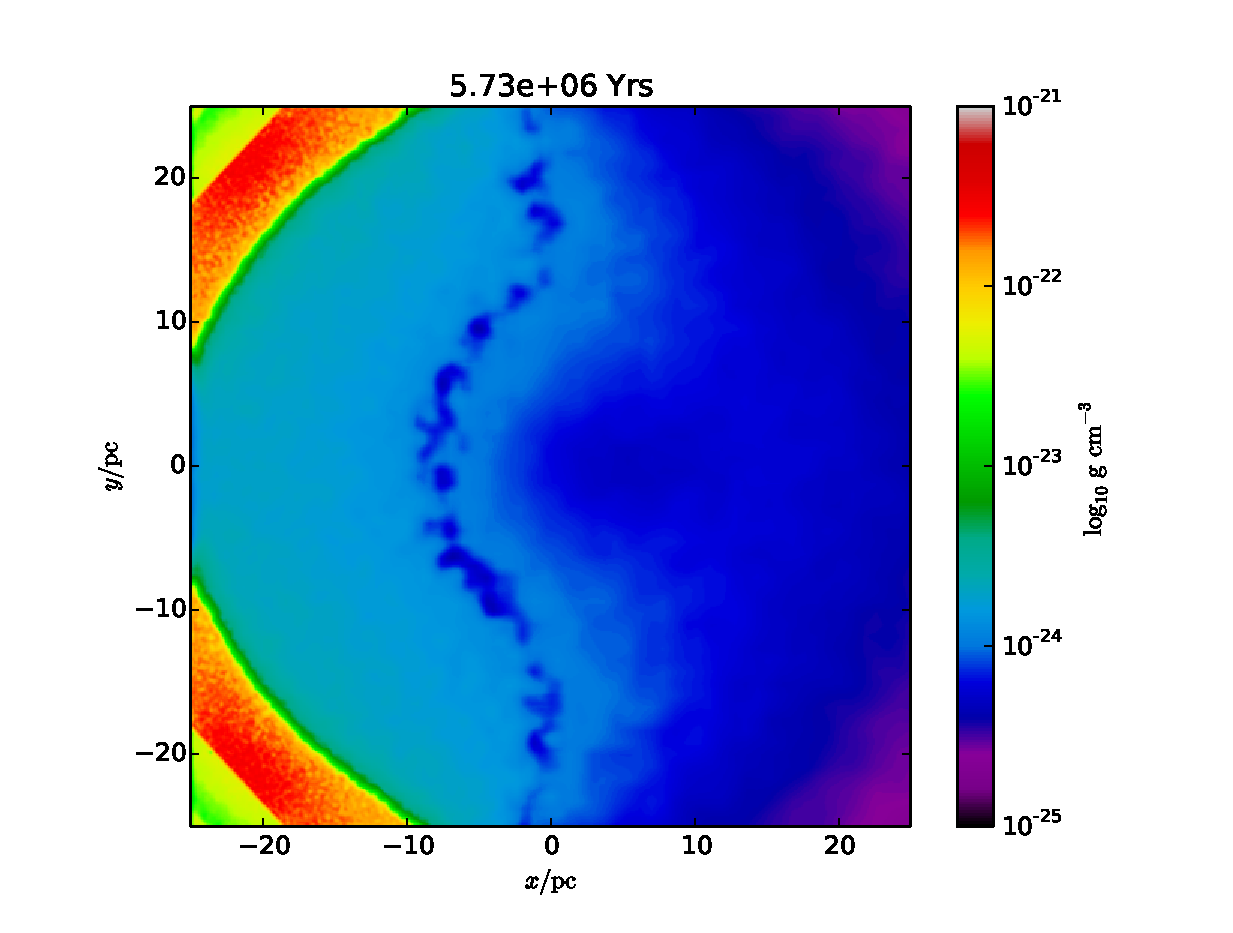
\includegraphics[width=\textwidth]{graphics/blister25600400rhoslice.eps}
                \caption{5 Myrs}
                \label{fig:champagne3}
        \end{subfigure}
        \caption[A champagne flow.]{The Blister HII region from \citet{gendelevKrumholz12}.}
        \label{fig:champagne}
\end{figure}

\section{Shadowing}
\label{sec:shadowing}

We present the shadowing test from \citet{hayesNorman03,gonzalezEt07,skinnerOstriker13}. A thin 2-D tube of gas with dimensions 0.12 cm tall x 1 cm long is irradiated from the left by a distance ((x,y) = (-100,0) cm) source with a characteristic temperature of 1740 K. The gas has an ambient density of $\rho_0 = 0.001 g cm^{-3}$ and an ambient temperature of 290 K. An oblate spheroid with dimensions $(x_0,y_0) = (0.1,0.06) cm$ is placed in the tube at $(x_c,y_c) = (0.5,0) cm$. The spheroid has a central density of $\rho_1 = 1000\rho_0 = 1 g cm^{-3}$ and the same ambient temperature. Note that hydrodynamics is turned off, so a mismatch in pressure is not an issue. The cloud has a density structure described by

\begin{equation}
\label{eq:shadowdensity}
\rho_{cloud}(x,y) = \rho_0 + \frac{(\rho_1 - \rho_0}){(1+e^{\Delta})},
\end{equation}

where

\begin{equation}
\label{eq:shadowdelta}
\Delta = 10\left\lbrace\left[\frac{x-x_c)}{x_0}\right]^2 + \left[\frac{y-y_c}{y_0}\right]^2-1\right\rbrace.
\end{equation}

This structure gives the cloud a ``fuzzy'' surface in that the density smoothly transitions rather than sharply jumps. The opacity is set as a function of density and temperature,

\begin{equation}
\label{eq:shadowopacity}
\kappa(T_{gas},\rho) = \kappa_0\left(\frac{T_{gas}}{T_0}\right)^{-3.5}\left(\frac{\rho}{\rho_0}\right),
\end{equation}

with $\kappa_0 = 100 cm^2 g^{-1}$. This gives an optical depth of 0.1 across the length of the box, excluding the dense cloud, and an optical depth of roughly 2000 across the diameter of the blob.

The tube is resolved by 280x80 SPH resolution elements, and the above density structure is obtained by changing the mass of the SPH particles (as opposed to increasing the number of particles). Note that this is not realistic for SPH, where higher densities are usually represented by a higher density of particles. However, we have elected to keep the same resolution as previous papers to aid in comparison.

At t = 0, the source is turned on and the simulation is evolved for 0.1 s, or $3\e{9}$ light crossing times. Figure \ref{fig:shadow} shows the simulation at t = 0.1 s.

\begin{figure}
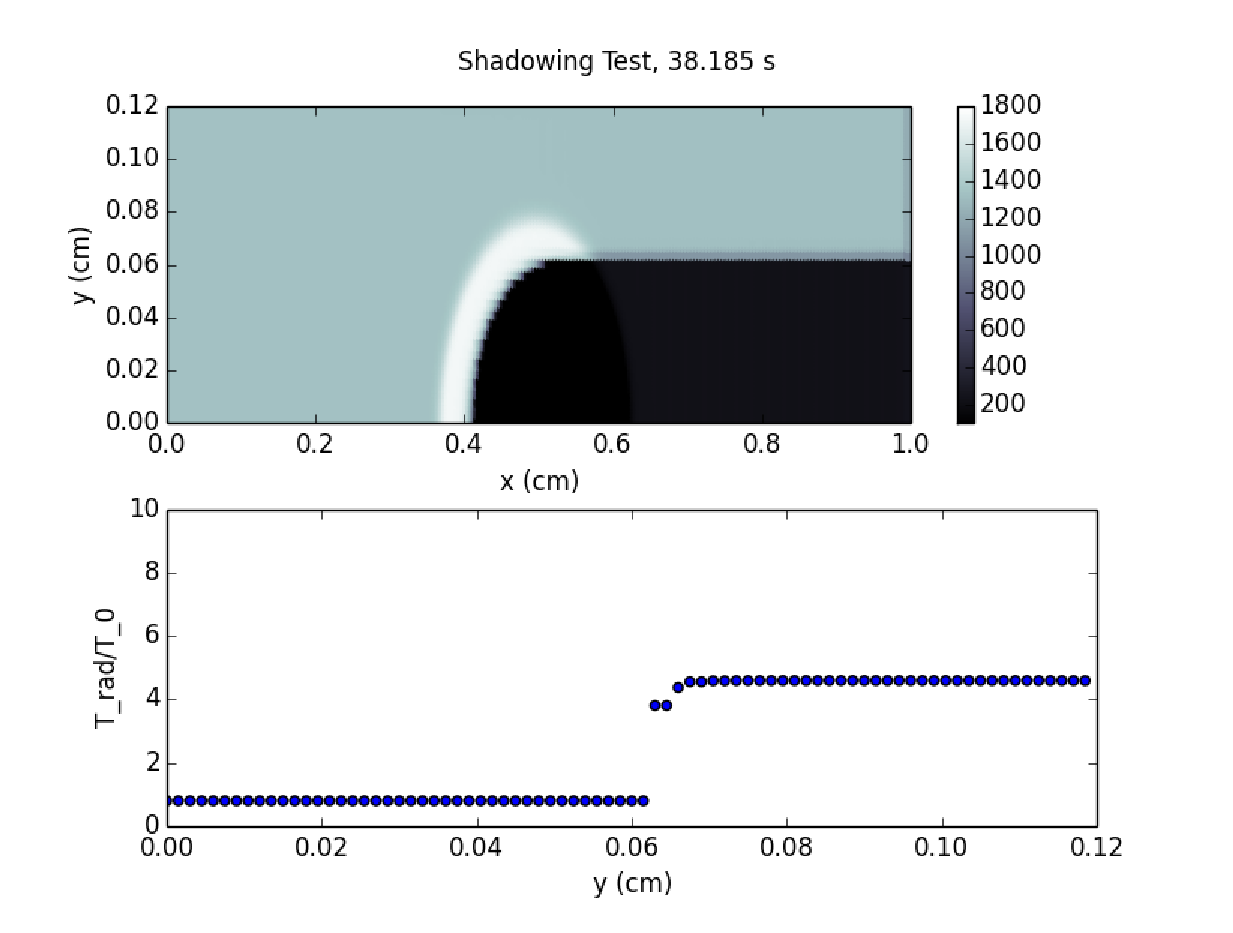
\includegraphics[width=\textwidth]{graphics/shadow10000.eps}
\caption[Shadowing.]{Demonstrating the codes ability to shadow.}
\label{fig:shadow}
\end{figure}

Need to fill in results...


\section{Ionization Front Trapping}
\label{sec:ifronttrapping}

Along the same lines of section \ref{sec:shadowing}, this section performs a shadowing test. However, this test includes ionizing radiation and is constructed in such a way that the ionization front should stall out inside of the dense sphere. The test is taken from \citet{ilievEt06}.

A 6.6 kpc cube is initiated with mean background density $2\e{-4} cm^{-3}$ and background temperature 8000 K. The dense clump is located at (x,y,z) = (5,3.3,3.3) and is given a density of 200 times the background, or 0.04 $cm^{-3}$, and a temperature of 40 K.

The conditions for trapping an ionization front are presented in \citet{shapiroEt04}. The authors show that a clump can trap an ionization front if

\begin{equation}
\label{eq:ifronttrap}
l_s = \frac{F}{\alpha n_H^2}
\end{equation}

is less than the diameter of the clump. In the above simulation $\alpha = 2.59\e{-13} (T/10^4 K)^(-3/4)$, which suggests the clump should trap the ionization front at $10^4$ somewhere around halfway through.

\begin{figure}
        \centering
        \begin{subfigure}[b]{0.3\textwidth}
                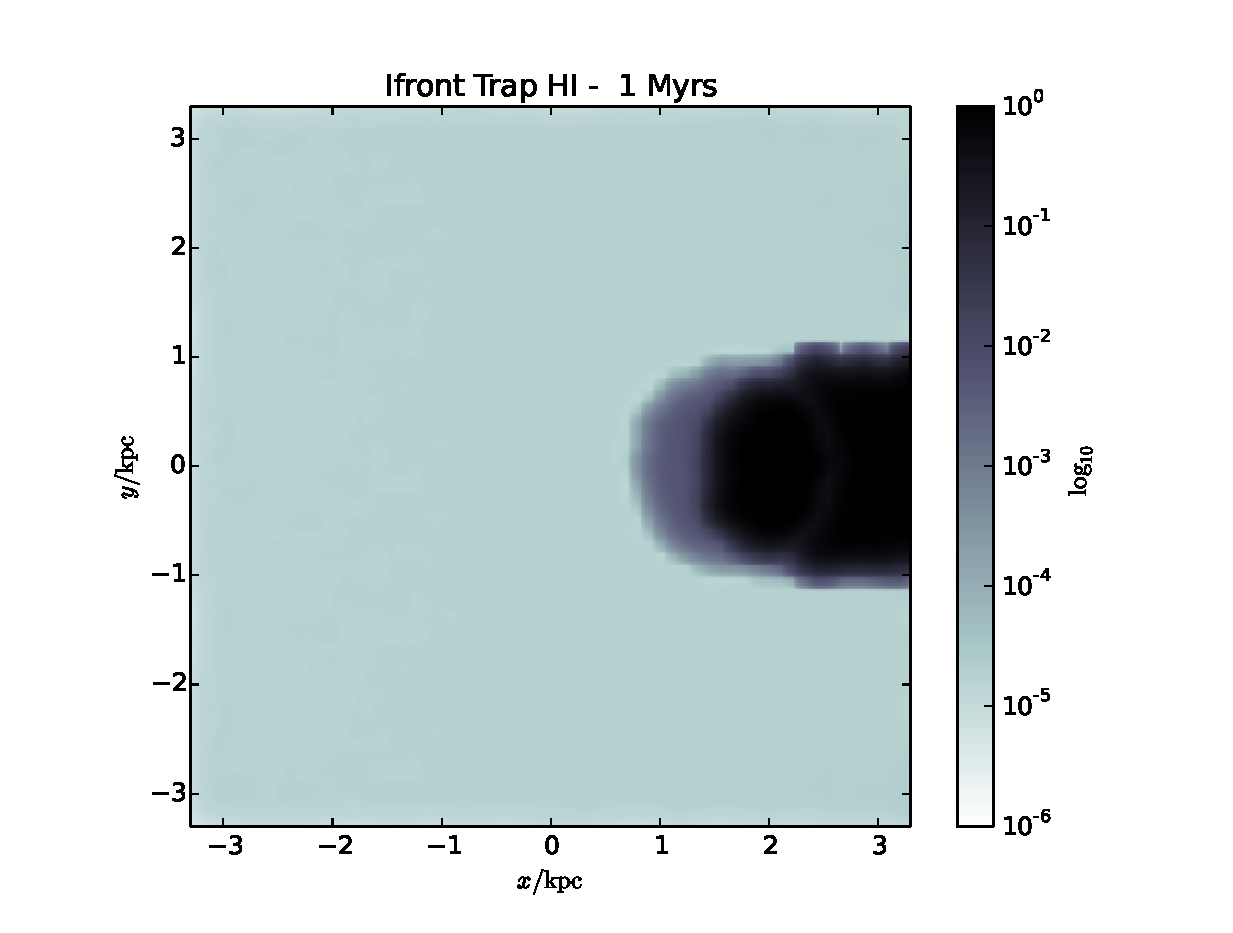
\includegraphics[width=\textwidth]{graphics/ifrontTrap00010HI.eps}
                \caption{HI, 1 Myr}
                \label{fig:ifronttrap1a}
        \end{subfigure}
        ~ 
        \begin{subfigure}[b]{0.3\textwidth}
                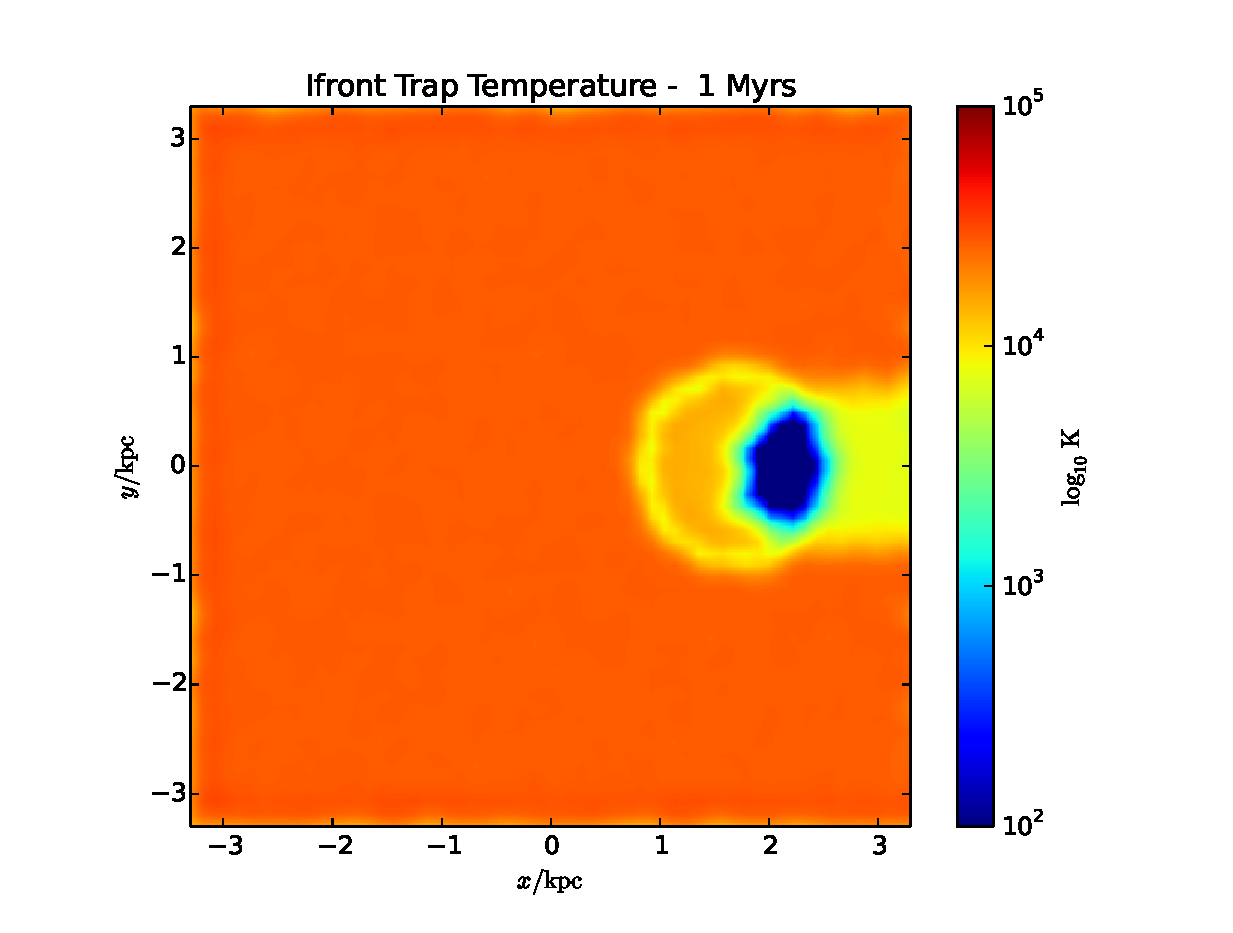
\includegraphics[width=\textwidth]{graphics/ifrontTrap00010Temp.eps}
                \caption{T, 1 Myr}
                \label{fig:ifronttrap1b}
        \end{subfigure}
        \caption[]{}
        \label{fig:ifronttrap1}
\end{figure}

\begin{figure}
        \centering
        \begin{subfigure}[b]{0.3\textwidth}
                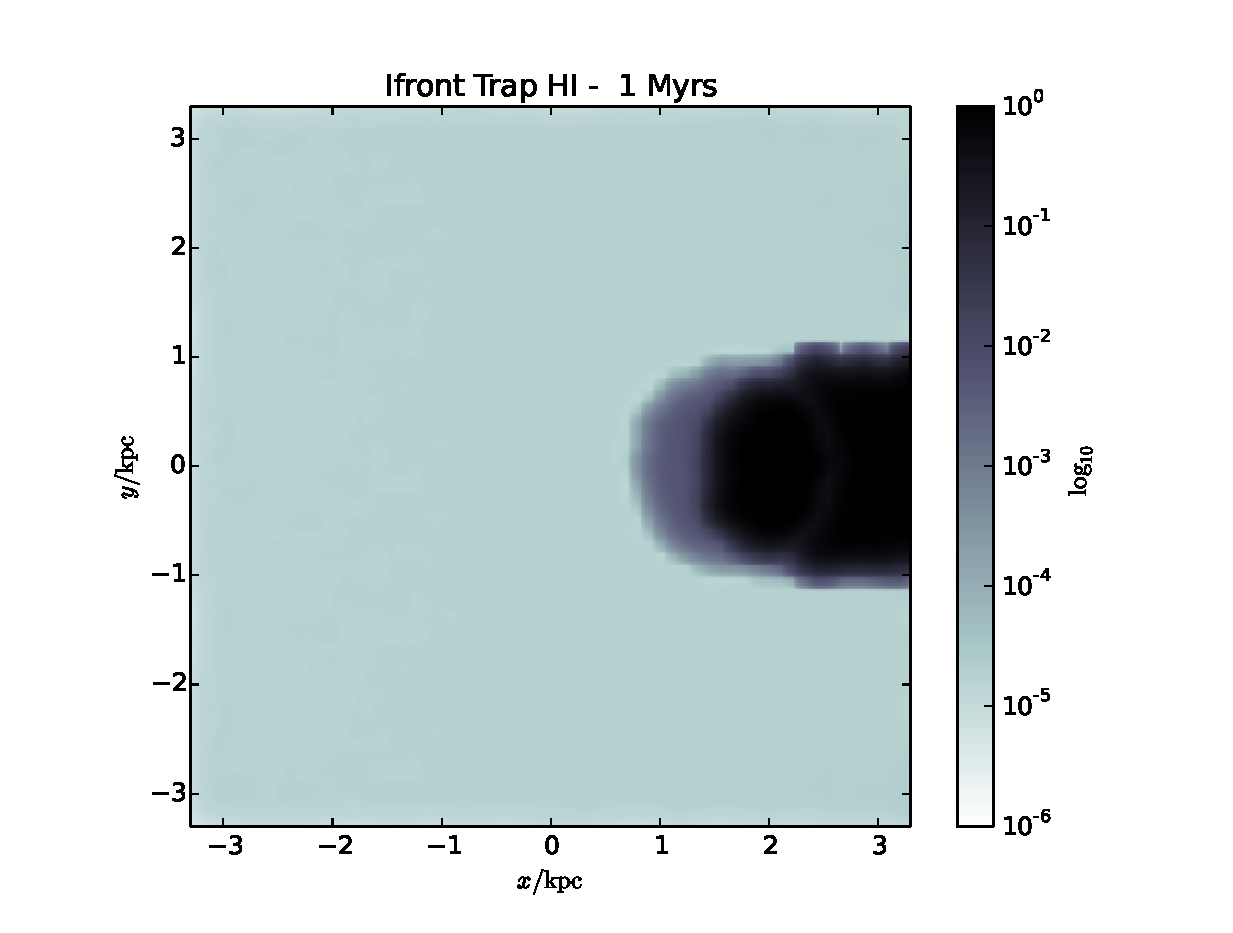
\includegraphics[width=\textwidth]{graphics/ifrontTrap00010HI.eps}
                \caption{HI, 1 Myr}
                \label{fig:ifronttrap2a}
        \end{subfigure}
        ~ 
        \begin{subfigure}[b]{0.3\textwidth}
                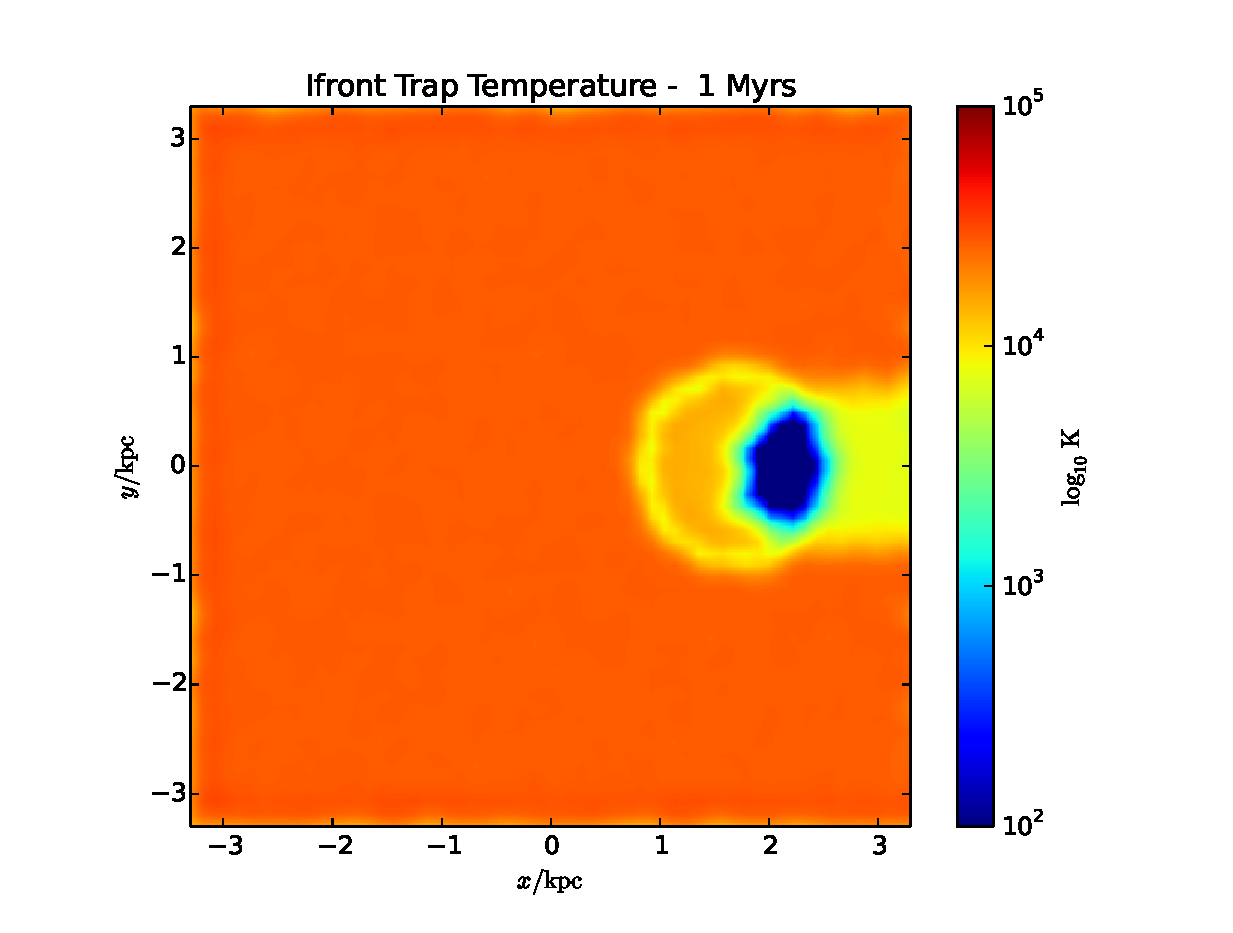
\includegraphics[width=\textwidth]{graphics/ifrontTrap00010Temp.eps}
                \caption{T, 15 Myrs}
                \label{fig:ifronttrap2b}
        \end{subfigure}
        \caption[]{}
        \label{fig:ifronttrap2}
\end{figure}


%Keep in mind that if a similar situation appeared in a simulation, the results would be improved due to a higher effective resolution in the dense clump.

%\section{Galaxy Disk}
%\label{sec:galaxydisk}
%
%Text to fix the formatting.

\section{Timings and Scaling}
\label{sec:timing}

Text to fix the formatting.

\begin{figure}
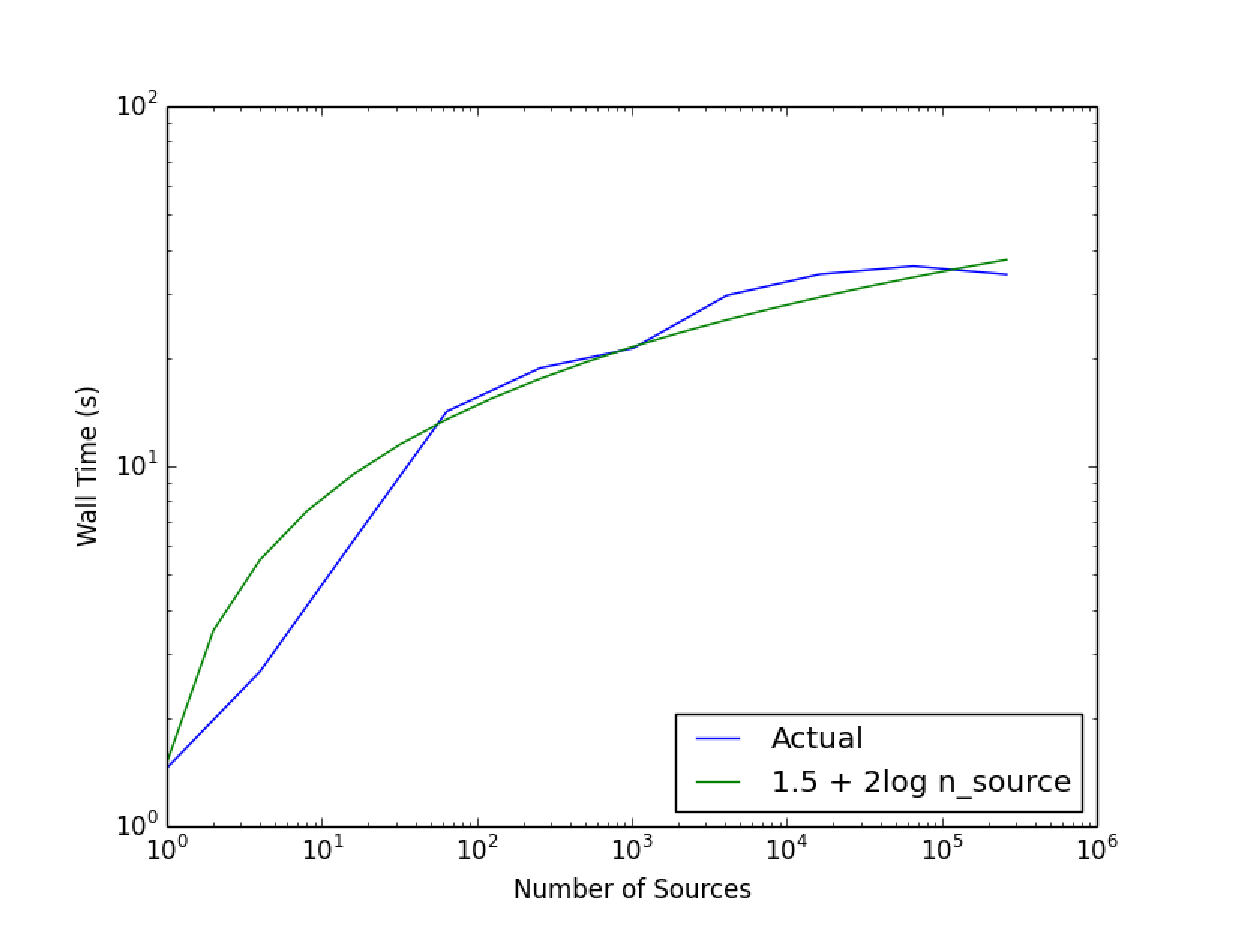
\includegraphics[width=\textwidth]{graphics/Timings.eps}
\caption[Wall time vs the number of sources.]{Wall time vs the number of sources.}
\label{fig:scaling}
\end{figure}

